% Springer Nature LaTeX template, December 2024 release.
% Intended journal: Foundations of Physics.
\documentclass[pdflatex,sn-mathphys-num]{sn-jnl}
\usepackage{graphicx}
\usepackage{amsmath,amssymb,amsfonts}
\usepackage{amsthm}
\usepackage{mathtools}
\usepackage{booktabs,tabularx,array}
\usepackage{enumitem}
\usepackage[title]{appendix}
\hypersetup{pdftitle={Relational Clock Transport Across Interaction Change: A Connected Jacobi Model},pdfauthor={Scott A. Jordan},pdfsubject={Relational observability of clock transport in a connected constrained Jacobi model},pdfkeywords={Relational dynamics, internal clocks, Jacobi action, complete observables, configuration-space geometry, interaction networks}}
\raggedbottom

\theoremstyle{thmstyleone}
\newtheorem{theorem}{Theorem}
\newtheorem{proposition}[theorem]{Proposition}
\newtheorem{lemma}[theorem]{Lemma}
\newcommand{\dd}{\mathrm d}
\newcommand{\e}{\mathrm e}
\newcommand{\R}{\mathbb R}
\newcommand{\Sone}{S^1}
\newcommand{\QED}{\hfill$\square$}

\begin{document}

\title[Relational Clock Transport Across Interaction Change]{Relational Clock Transport Across Interaction Change: A Connected Jacobi Model}

\author*[1]{\fnm{Scott A.} \sur{Jordan}}\email{scott@simplelogicsolutions.com}

\affil*[1]{\orgname{Independent researcher}, \orgaddress{\city{Fayetteville}, \state{North Carolina}, \country{USA}}; \href{https://orcid.org/0009-0005-7444-3386}{ORCID: 0009-0005-7444-3386}}

\abstract{The foundational question addressed here is not whether a variable kinetic coefficient changes a clock rate, but when a comparison of clocks across different interaction organizations has invariant relational meaning at all. In disconnected sectors the comparison is empty because each sector admits an independent recalibration. We construct a connected, reparameterization-invariant Jacobi model in which the same two compact phase clocks are transported through a continuous interaction-link change. Their conserved phase charges define branch-local complete observables on selected organization surfaces. The principal result is an observability theorem: once clock identity, unit-cycle normalization, connected transport, and preparation are fixed, the endpoint double ratio survives gauge reduction and is nontrivial exactly when the two clock fibers undergo unequal fractional changes. The elementary variable-inertia identity used in the calculation is not itself the novelty. Uninterrupted charge transport, endpoint rate resetting, and equal-energy preparation are shown to be different experiments. A clock-preserving non-removability proposition establishes that a nonconstant fiber circumference cannot be flattened by a degree-one diffeomorphism preserving the specified $2\pi$ cycle; integer rescalings of magnitude greater than one are covering maps, not such diffeomorphisms. A positive graph-Laplacian block separately weights changes of active particle-separation records and vanishes on particle-co-moving histories. The construction also shows that a universal fractional clock response is invisible to local two-clock ratios, delimiting what a future universal ``progression'' factor could mean operationally. The model establishes a finite relational observability result, not a universal clock law or a theory of spacetime or gravity.}

\keywords{Relational dynamics, internal clocks, Jacobi action, complete observables, configuration-space geometry, interaction networks}

\maketitle

\section{Introduction: the clock-calibration problem}

A physical clock is a material subsystem whose reading is inferred from a repeatable record. In a generally covariant or reparameterization-invariant description, such a record can label correlations without supplying an external physical time. Jacobi actions, best matching, partial and complete observables, and changes of internal clock provide established frameworks for making those correlations gauge invariant \cite{BarbourBertotti,Rovelli,Dittrich2006,Dittrich2007,AndersonBook,HohnVanrietvelde,HohnTrinity}.

A more specific problem arises when the organization of the interacting system changes. Suppose a clock is assigned one effective kinetic coefficient in an open interaction network and another in a closed network. If the two organizations are represented by disconnected sectors, each sector can be flattened by an independent clock-coordinate rescaling. A comparison then has no invariant content until one stipulates how the clocks and their canonical data are identified across sectors. Equal momenta, equal rates, and equal clock energies are physically distinct preparation rules and generally produce different endpoint ratios.

The central question is therefore
\begin{quote}
\emph{Under what conditions does an interaction-dependent clock comparison survive gauge freedom, independent calibration, and preparation ambiguity as a relational observable?}
\end{quote}
The question is prior to any proposed clock law. Conservation of phase momentum with a variable inertia already gives the familiar mechanical relation $\dot\theta\propto I^{-1}$. What requires proof is that a comparison based on that relation refers to the same operational clocks at two relationally selected events, uses one physically stated transport protocol, and cannot be erased by an admissible clock-preserving redefinition.

Three distinctions are essential. First, a gauge transformation changes the description of one physical history, whereas resetting a clock changes the history or its preparation. Second, a coordinate redefinition of a compact phase is not automatically an equivalence of clock constructions: one physical cycle is part of the operational identification. Third, persistent interaction organization and departure from particle co-motion are different structures. A network may reorganize while particle separations remain fixed, and particles may change their relational separations within a fixed organizational state.

This paper treats those distinctions as design requirements. Open and closed organizations are embedded in one connected configuration space, the same two compact phase clocks are transported through a continuous interaction-link activation, and their momenta are conserved Noether charges of one action. Departure from particle co-motion is represented separately by a positive graph-Laplacian quadratic form on relational differentials. The model replaces an arbitrary cross-sector calibration rule by a dynamical transport protocol on one gauge orbit. It does not make all protocols equivalent: uninterrupted transport, endpoint rate resetting, and equal-energy preparation remain different experiments. Dynamical interaction links also place the model near the broad class of adaptive or coevolving networks, although the present use is a finite mechanical construction rather than a network-evolution theory \cite{GrossBlasius}.

The principal result, Theorem~\ref{thm:transport}, is operational rather than kinematic. A cross-organization comparison that is arbitrary in disconnected sectors becomes a well-defined branch-local complete observable when the same normalized compact clock fibers and conserved charges are transported through one connected constrained history. The double ratio is nontrivial exactly when the fibers undergo unequal fractional changes. Proposition~\ref{prop:nonremove} then proves that this result is not removable by a degree-one clock-preserving diffeomorphism. A supporting variational result shows that, on every fixed regular stationary branch, the stationary abbreviated action is nondecreasing in the coefficient of the positive active-link block, with equality exactly for particle co-motion.

The scope is deliberately finite. The model does not derive its effective coefficients from microscopic clock dynamics, a universal temporal standard, a local field-theory constraint algebra, a causal cone, quantum dynamics, or metric gravity. Its purpose is to establish precisely when interaction-dependent clock geometry and particle-co-motion loading are consistent and observable after calibration, preparation, gauge, and frame-dependence objections are made explicit.

\section{Relational clocks, gauge, and preparation}

\subsection{Inherited machinery and the restricted claim}

A degree-one Jacobi action is already a geodesic principle on configuration space \cite{Arnold}. Best matching already removes designated configurational redundancies, and complete observables already construct gauge-invariant correlations in constrained systems \cite{Dittrich2006,Dittrich2007}. Clock-neutral formulations explain how distinct reduced clock descriptions can be related through a common constrained description \cite{HohnVanrietvelde,HohnTrinity}. Relational particle models provide established finite arenas for these issues \cite{AndersonRPM}. Weighted graph Laplacians and their consensus null spaces are likewise standard structures in spectral graph theory and network dynamics \cite{Chung,OlfatiSaber}.

The proposed contribution is not a new graph-theoretic null-space theorem, a new general theory of complete observables, or the identity $I\dot\theta=\mathrm{const}$. It is the combined observability result obtained by placing two interaction-dependent blocks in one connected relational Jacobi metric: a clock-fiber block that responds to persistent organization and an active-link block that responds to changes of particle-separation records. The same clocks, their normalized cycles, their conserved canonical data, and the preparation protocol are carried through one constrained history. Table~\ref{tab:scope} separates inherited tools from the restricted additions.

\begin{table}[ht]
\centering
\small
\begin{tabularx}{\textwidth}{@{}>{\raggedright\arraybackslash}X>{\raggedright\arraybackslash}X@{}}
\toprule
Element & Status in this paper\\
\midrule
Degree-one Jacobi action and Hamiltonian constraint & Established relational-mechanics structure\\
Translation best matching and complete observables & Established constrained-system framework\\
Weighted graph Laplacian and connected-component null space & Established graph-theoretic structure\\
Variable-inertia identity $I\dot\theta=\mathrm{const}$ & Elementary mechanical input, not the novelty\\
Continuous interaction-link coordinate in one phase space & Model choice introduced here\\
Interaction-dependent compact clock fibers & Proposed persistent-organization coupling\\
Active-link quadratic form on relational differentials & Proposed particle-non-co-motion coupling\\
Same-orbit transport with fixed clock identity and protocol & Principal relational-clock construction\\
Gauge-invariant endpoint theorem and clock-preserving non-removability & Principal foundations results\\
Universal clocks, spacetime locality, and metric gravity & Open correspondence problems\\
\bottomrule
\end{tabularx}
\caption{Established structures and the restricted contribution of the model.}
\label{tab:scope}
\end{table}

Because the clocks used below are compact phases, each is a locally monotonic record only after one cycle has been lifted to the universal cover. Periodic clocks require greater care than globally monotonic clocks, and naive winding counting does not supply a global Dirac observable without additional structure \cite{Chataignier}. All complete-observable statements below are therefore branch local.

\subsection{Operational clock identity}

A clock construction consists here of a compact orbit, its orientation, and the identification of one complete orbit with one operational cycle. For the $i$th clock this is a specified $U(1)$ action generated by
\begin{equation}
k_i=\frac{\partial}{\partial\theta_i},\qquad \theta_i\sim\theta_i+2\pi.
\end{equation}
A shift of phase origin, an orientation-preserving reparameterization of the system orbit, or a global particle translation does not change that clock. A transformation that changes which closed curve counts as one cycle changes the clock construction rather than merely its coordinates. This distinction is used in Sec.~\ref{sec:invariance} to separate clock-preserving equivalences from physical recalibration.

\subsection{Preparation is physical input}

A clock comparison is incomplete until its preparation protocol is specified. In the connected model, the natural protocol is uninterrupted transport: the same two clock degrees of freedom evolve on one gauge orbit with no external intervention on their $U(1)$ charges. An independently prepared endpoint experiment can instead impose equal angular rates or equal individual clock energies. These preparations are not gauge choices. They alter canonical data and therefore answer different physical questions.

\section{General connected Jacobi construction}

Let $q^A$ be dimensionless coordinates on a configuration manifold $Q$. A group $G$ represents descriptive redundancy, with infinitesimal generators $\xi_\alpha^A(q)$. The best-matched differential is
\begin{equation}
Dq^A=\dd q^A-\dd g^\alpha\,\xi_\alpha^A(q).
\end{equation}
Let $G_{AB}(q)$ be a positive metric and
\begin{equation}
\Omega(q)=E-V(q)>0
\end{equation}
throughout the history. The Jacobi action is
\begin{equation}
S_J=S_0\int\dd\lambda\,\sqrt{2\Omega(q)G_{AB}(q)D_\lambda q^A D_\lambda q^B}.
\end{equation}
Homogeneity of degree one makes the arbitrary label $\lambda$ physically irrelevant. An equivalent einbein action is
\begin{equation}
S_E=\frac{S_0}{2}\int\dd\lambda\left[N^{-1}G_{AB}D_\lambda q^A D_\lambda q^B+2N(E-V)\right].
\end{equation}
With dimensionless momenta $p_A=P_A/S_0$, variation with respect to $N$ gives
\begin{equation}
\mathcal H=\frac12G^{AB}p_Ap_B+V-E\approx0,
\end{equation}
while free-endpoint variation of the best-matching variables gives
\begin{equation}
\mathcal J_\alpha=p_A\xi_\alpha^A\approx0.
\end{equation}

\subsection{Persistent organization and particle co-motion}

Let $u$ be invariant under the configurational gauge group $G$ and describe a continuous interaction change. It is not, in general, a Dirac observable of the Hamiltonian constraint: under Hamiltonian flow it is a partial observable that can serve as a branch-local relational label. Let $C(u)$ be a coarse-grained organization descriptor entering an effective metric. No identification with entropy, algorithmic complexity, or a complete microscopic interaction count is assumed.

Let $R_e(q)$ denote the particle-separation record carried by an active interaction channel $e$. Exact particle co-motion on a history segment means
\begin{equation}
DR_e=0
\end{equation}
for every active channel on that segment. This definition invokes neither coordinate velocity nor a preferred frame. For nonnegative active-link weights $w_e(q)$, define
\begin{equation}
\dd M^2=\sum_e w_e(q)(DR_e)^2.
\end{equation}
This form is positive semidefinite and vanishes exactly when all positively weighted particle-separation records are unchanged. For a graph with incidence matrix $B$ and diagonal weight matrix $W$,
\begin{equation}
\dd M^2=\dd y^{T}L\dd y,\qquad L=B^TWB.
\end{equation}

\begin{proposition}[Active-link co-motion null space]
For nonnegative link weights, $\dd M^2=0$ if and only if the particle displacement is constant on each connected component of the positively weighted graph. If the active graph is connected, the only null direction is global translation, and $\dd M^2$ is positive definite after translation reduction.
\end{proposition}
\noindent\emph{Proof.} The form is a sum of nonnegative weighted squares. It vanishes exactly when the displacement difference on every positively weighted edge vanishes. Equality propagates along every path in a connected component. The converse is immediate. \QED

Persistent organization and particle co-motion are therefore logically distinct. The link variable $u$ and organization scalar $C(u)$ may change while $DR_e=0$. Full network stasis is the stronger condition $DR_e=0$ for all active edges together with $\dd u=0$.

\subsection{General compact clock fibers}

Take two compact phase clocks with arbitrary positive inertias
\begin{equation}
\theta_i\in S^1,\qquad I_i(u)>0,\qquad i=1,2.
\end{equation}
Their clock-sector line element is
\begin{equation}
\dd\Sigma_{\rm clock}^2=I_1(u)\dd\theta_1^2+I_2(u)\dd\theta_2^2.
\end{equation}
The central transport result is derived for these general functions before any particular coupling ansatz is imposed.

\section{A minimal interaction-network model}

\subsection{Configuration space and continuous link activation}

Consider three distinguishable particles on a line with coordinates $y_a$, $a=1,2,3$. The links 12 and 23 are permanently active. A dimensionless coordinate $u\in\R$ controls the strength of the additional 31 channel. The organization window is
\begin{equation}
0\le u\le1,\qquad u=0\ \text{open chain},\qquad u=1\ \text{fully activated closure link}.
\end{equation}
The process is a continuous activation of one interaction channel, not a singular change in the topology of configuration space. The kinematic space is
\begin{equation}
Q=\R_y^3\times\R_u\times S^1_{\theta_1}\times S^1_{\theta_2}.
\end{equation}
Only global translations are gauge:
\begin{equation}
y_a\mapsto y_a+\epsilon,\qquad u\mapsto u,\qquad\theta_i\mapsto\theta_i.
\end{equation}
No claim of scale, reflection, particle-relabeling, or full Euclidean-frame invariance is made.

On the physical branch, assign
\begin{equation}
w_{12}=1,\qquad w_{23}=1,\qquad w_{31}=u^2.
\end{equation}
The active-link form is then
\begin{equation}
\dd M^2=\dd y^TL(u)\dd y=(\dd y_1-\dd y_2)^2+(\dd y_2-\dd y_3)^2+u^2(\dd y_3-\dd y_1)^2.
\end{equation}
The permanent links keep the graph connected throughout $0\le u\le1$. For an explicit organization descriptor, choose
\begin{equation}
C(u)=2+(1+\kappa)u^2,\qquad\kappa>-1.
\end{equation}
The constant term records the two permanent channels, and the nonnegative $u^2$ contribution records the activated closure channel and its cycle contribution. This simple expression is a model choice, not a uniqueness claim.

\subsection{Effective phase-clock ansatz}

To embed the phase metric in a larger effective clock sector, introduce complex variables
\begin{equation}
\psi_i=r_i\e^{\mathrm i\theta_i}
\end{equation}
with clock-sector kinetic line element and radial potential
\begin{align}
\dd\Sigma_{\rm clock}^2&=\sum_{i=1}^2[M_i+g_iC(u)]\dd\psi_i^*\dd\psi_i,\\
U_{r,i}(r_i)&=\frac{m_{r,i}^2}{2}(r_i-r_{i0})^2+O[(r_i-r_{i0})^3].
\end{align}
When the radial modes are heavy relative to the organization-change scale, restriction to the low-energy phase submanifold gives
\begin{equation}
I_i(u)=r_{i0}^2[M_i+g_iC(u)],\qquad M_i+g_iC(u)>0.
\end{equation}
The fractional response is
\begin{equation}
\chi_i(C)=\frac{\dd\ln I_i}{\dd C}=\frac{g_i}{M_i+g_iC}.
\end{equation}
This is an effective kinetic-coupling ansatz. Whether realistic clocks possess such couplings, or flow toward a universal low-energy response, is not decided here.

\subsection{Metric, potential, and reduction}

Let $m,K,B_V>0$ and $\mu\ge0$. Choose
\begin{equation}
V(u)=B_Vu^2(1-u)^2.
\end{equation}
The best-matched kinetic metric is
\begin{equation}
\dd\Sigma^2=m\sum_{a=1}^3(\dd y_a-\dd g)^2+\mu\dd M^2+K\dd u^2+I_1(u)\dd\theta_1^2+I_2(u)\dd\theta_2^2.
\end{equation}
The $I_i$ terms encode persistent organization in the clock sector. The $\mu\dd M^2$ term encodes the additional metric cost of changing active particle-separation records. Exact particle co-motion removes the latter term but not the former.

Before reduction, the constraints are
\begin{align}
\mathcal J&=p_1+p_2+p_3\approx0,\\
\mathcal H&=\frac12p^TG_y(u)^{-1}p+\frac{p_u^2}{2K}+\frac{\pi_1^2}{2I_1(u)}+\frac{\pi_2^2}{2I_2(u)}+V(u)-E\approx0,
\end{align}
where $G_y(u)=m\mathbf1+\mu L(u)$. Translation invariance gives $\{\mathcal H,\mathcal J\}=0$; the two constraints are first class. This is a finite global consistency check, not an analogue of the continuum hypersurface-deformation algebra.

Introduce Jacobi coordinates
\begin{equation}
R=\frac{y_1+y_2+y_3}{\sqrt3},\qquad \rho=\frac{y_2-y_1}{\sqrt2},\qquad \xi=\frac{y_1+y_2-2y_3}{\sqrt6}.
\end{equation}
The translation constraint is $p_R=0$. The fixed orthogonal rotation
\begin{equation}
x=\frac{\sqrt3\rho+\xi}{2},\qquad z=\frac{-\rho+\sqrt3\xi}{2}
\end{equation}
then gives
\begin{equation}
\dd M^2=3\dd x^2+(1+2u^2)\dd z^2.
\end{equation}
Thus
\begin{equation}
A_x=m+3\mu,\qquad A_z(u)=m+\mu(1+2u^2),
\end{equation}
and the reduced Hamiltonian constraint is
\begin{equation}
\mathcal H_{\rm red}=\frac{p_x^2}{2A_x}+\frac{p_z^2}{2A_z(u)}+\frac{p_u^2}{2K}+\frac{\pi_1^2}{2I_1(u)}+\frac{\pi_2^2}{2I_2(u)}+V(u)-E\approx0.
\end{equation}
The cyclic momenta $p_x,p_z,\pi_1,\pi_2$ are constants of motion. Define
\begin{align}
E_x&=\frac{p_x^2}{2A_x},\\
V_{\rm eff}(u)&=V(u)+\frac{p_z^2}{2A_z(u)}+\frac{\pi_1^2}{2I_1(u)}+\frac{\pi_2^2}{2I_2(u)},\\
E_u&=E-E_x.
\end{align}
A monotonic orbit connects $u_-$ to $u_+$ whenever
\begin{equation}
E_u>\max_{u\in[u_-,u_+]}V_{\rm eff}(u).
\end{equation}
With $\varepsilon=\operatorname{sgn}p_u$, the orbit is determined by quadratures:
\begin{align}
\sigma-\sigma_0&=\varepsilon\sqrt{\frac K2}\int_{u_0}^{u}\frac{\dd v}{\sqrt{E_u-V_{\rm eff}(v)}},\\
\theta_i(u)-\theta_{i0}&=\varepsilon\pi_i\sqrt{\frac K2}\int_{u_0}^{u}\frac{\dd v}{I_i(v)\sqrt{E_u-V_{\rm eff}(v)}},\\
z(u)-z_0&=\varepsilon p_z\sqrt{\frac K2}\int_{u_0}^{u}\frac{\dd v}{A_z(v)\sqrt{E_u-V_{\rm eff}(v)}}.
\end{align}

\section{Co-motion loading and stationary-action monotonicity}

The active-link term is not only a definition of relational change; it contributes to the invariant Jacobi length.

\begin{proposition}[Stationary-action monotonicity]
Let $\gamma_\mu$ be a differentiable family of stationary histories with fixed relational endpoints, all within one winding or homotopy class. Assume a regular Jacobi denominator and no branch crossing or caustic on the family. If
\begin{equation}
G_{AB}^{(\mu)}=G_{AB}^{(0)}+\mu M_{AB},\qquad M_{AB}\dot q^A\dot q^B\ge0,
\end{equation}
then on that stationary branch
\begin{equation}
\frac{\partial S_{\rm on}}{\partial\mu}=S_0\int\dd\lambda\,
\frac{\Omega(q)M_{AB}\dot q^A\dot q^B}{\sqrt{2\Omega(q)G_{CD}^{(\mu)}\dot q^C\dot q^D}}\ge0.
\end{equation}
For the connected three-particle model, equality holds if and only if $\dot x=\dot z=0$ almost everywhere, namely particle co-motion modulo translation.
\end{proposition}
\noindent\emph{Proof.} Differentiate the action with respect to $\mu$. The implicit variation of the stationary history contributes an Euler-Lagrange term and a fixed-endpoint term, both zero. The remaining explicit derivative gives the displayed expression. Here
\begin{equation}
M_{AB}\dot q^A\dot q^B=3\dot x^2+(1+2u^2)\dot z^2,
\end{equation}
which vanishes precisely when both reduced shape differentials vanish. \QED

This is a branchwise envelope-theorem statement. It does not compare independently prepared moving and co-moving experiments, and it does not imply monotonicity of the globally minimizing branch if different stationary branches exchange dominance. Persistent organization $C(u)$ and the link coordinate $u$ may remain nontrivial when the active-link contribution vanishes.

For $p_z\ne0$, a local clock-versus-shape comparison is
\begin{equation}
R_{iz}(u)=\frac{\dd\theta_i}{\dd z}=\frac{\pi_i/I_i(u)}{p_z/A_z(u)}=\frac{\pi_iA_z(u)}{p_zI_i(u)}.
\end{equation}
The two interaction effects are distinct: $I_i(u)$ carries persistent clock response, while $A_z(u)$ carries active-link particle-non-co-motion loading. Under exact particle co-motion, $p_x=p_z=0$ and no particle-shape clock is available; the $\mu$ term drops out of the remaining clock-link dynamics.

\section{Complete observables and relational clock transport}

\subsection{Complete observables on monotonic branches}

Let $\alpha_{\mathcal H}^s$ denote the Hamiltonian flow generated by $\mathcal H_{\rm red}$. On a branch where the lifted phase $T_i=\theta_i\in\widetilde\R$ is monotonic,
\begin{equation}
\{T_i,\mathcal H_{\rm red}\}=\frac{\pi_i}{I_i(u)}\ne0.
\end{equation}
Let $s_i(x,\tau)$ be the local solution of
\begin{equation}
\alpha_{\mathcal H}^{s_i(x,\tau)}T_i(x)=\tau.
\end{equation}
For a phase-space function $f$, define
\begin{equation}
F_{f\mid T_i}(\tau)(x)=\alpha_{\mathcal H}^{s_i(x,\tau)}f(x).
\end{equation}

\begin{lemma}[Dirac property]
On every branch on which $T_i$ is monotonic and the inverse is single valued,
\begin{equation}
\{F_{f\mid T_i}(\tau),\mathcal H_{\rm red}\}\approx0.
\end{equation}
\end{lemma}
\noindent\emph{Proof.} A gauge displacement by $\epsilon$ changes the required flow parameter according to $s_i(\alpha_{\mathcal H}^{\epsilon}x,\tau)=s_i(x,\tau)-\epsilon$. The complete observable is therefore constant along the Hamiltonian gauge orbit. Differentiation at $\epsilon=0$ gives the result. \QED

Using the quadrature above, define $\Theta_i(u;u_0)$ as the lifted phase along the orbit. Then
\begin{equation}
F_{u\mid T_i}(\tau)=\Theta_i^{-1}(\tau;u_0),\qquad
F_{T_j\mid T_i}(\tau)=\Theta_j\bigl(\Theta_i^{-1}(\tau;u_0);u_0\bigr).
\end{equation}
On a segment where both clocks are monotonic, selecting an event with $T_1$ and then changing to $T_2$ selects the same point on the same gauge orbit. This is the standard complete-observable consistency condition, not a new theorem of clock neutrality.

The same construction applies when $u$ is monotonic. Although $u$ is invariant under translations, it changes along Hamiltonian gauge flow and is therefore a partial observable. For any phase-space scalar $r$, define
\begin{equation}
F_{r\mid u}(u_*)=\alpha_{\mathcal H}^{s_u(x,u_*)}r(x),\qquad
\alpha_{\mathcal H}^{s_u(x,u_*)}u(x)=u_*.
\end{equation}
It obeys $\{F_{r\mid u}(u_*),\mathcal H_{\rm red}\}\approx0$ on the chosen monotonic branch.

\subsection{Kinematic identity versus the observability result}

The phase-shift symmetries generate conserved Noether charges
\begin{equation}
Q_i=S_0\pi_i=S_0I_i(u)\frac{\dot\theta_i}{N},\qquad \frac{\dd Q_i}{\dd\lambda}=0.
\end{equation}
Let
\begin{equation}
\eta_i=\frac{\dd\theta_i}{2\pi},\qquad\oint_{S_i^1}\eta_i=1
\end{equation}
be the normalized cycle one-form. Its pullback to an orbit gives the local cycle rate $\nu_i=\dot\theta_i/(2\pi)$. The local ratio
\begin{equation}
r_{12}=\frac{\nu_1}{\nu_2}=\frac{\dot\theta_1}{\dot\theta_2}=\frac{\pi_1I_2(u)}{\pi_2I_1(u)}
\label{eq:kinematic}
\end{equation}
is a partial observable. Equation~\eqref{eq:kinematic} is the familiar variable-inertia identity. By itself it neither solves the cross-sector calibration problem nor proves that a clock comparison is gauge invariant. The foundations result begins only after clock identity, connected transport, relational event selection, and preparation are supplied.

On a branch where $u$ is monotonic, the conditional complete observable is
\begin{equation}
R_{12\mid u}(u_*):=F_{r_{12}\mid u}(u_*)=\frac{\pi_1I_2(u_*)}{\pi_2I_1(u_*)},\qquad
\{R_{12\mid u}(u_*),\mathcal H_{\rm red}\}\approx0.
\end{equation}

\begin{theorem}[Connected relational clock transport]
\label{thm:transport}
Consider one regular gauge orbit that crosses the relational surfaces $u=u_-$ and $u=u_+$. Suppose (i) the two compact clock actions, orientations, and normalized unit cycles are fixed throughout the connected history; (ii) $u$ is monotonic between the selected surfaces; and (iii) no intervention changes the conserved phase charges. Then
\begin{equation}
\Xi_{+-}:=\frac{R_{12\mid u}(u_+)}{R_{12\mid u}(u_-)}
=\frac{I_2(u_+)/I_2(u_-)}{I_1(u_+)/I_1(u_-)}
\label{eq:Xi}
\end{equation}
is a branch-local Dirac observable, independent of the arbitrary orbit parameter and of the initial charge ratio $\pi_1/\pi_2$. Moreover,
\begin{equation}
\Xi_{+-}=1\quad\Longleftrightarrow\quad\Delta\ln I_1=\Delta\ln I_2,
\end{equation}
so uninterrupted relative clock transport is nontrivial exactly when the two clock fibers undergo unequal fractional changes.
\end{theorem}
\noindent\emph{Proof.} Each $R_{12\mid u}(u_*)$ is a complete observable and hence is constant on the Hamiltonian gauge orbit. Their ratio is therefore also a Dirac observable. Conservation of the same $\pi_i$ between the two relational events cancels the charge ratio and yields Eq.~\eqref{eq:Xi}. Taking its logarithm gives $\ln\Xi_{+-}=\Delta\ln I_2-\Delta\ln I_1$, which proves the criterion. \QED

The theorem is the paper's principal result. The elementary identity \eqref{eq:kinematic} is necessary input, but the content of the theorem is that the endpoint comparison remains meaningful after the relevant gauge, calibration, cycle-identification, and protocol requirements are imposed.

For the linear effective ansatz,
\begin{equation}
\Xi_{+-}=\frac{[M_2+g_2C_+][M_1+g_1C_-]}{[M_1+g_1C_+][M_2+g_2C_-]},\qquad C_\pm=C(u_\pm),
\end{equation}
and, when $C_+\ne C_-$,
\begin{equation}
\Xi_{+-}\ne1\quad\Longleftrightarrow\quad g_2M_1\ne g_1M_2.
\end{equation}
In the weak-coupling regime,
\begin{equation}
\ln\Xi_{+-}=\left(\frac{g_2}{M_2}-\frac{g_1}{M_1}\right)(C_+-C_-)+O(g_i^2).
\end{equation}
The surface $g_1/M_1=g_2/M_2$ is the exact relative-clock no-effect condition for this ansatz. Organization may still affect the common geometry and link dynamics even though the differential two-clock signal vanishes. In the present diagonal model the transport is integrable and endpoint dependent. No nontrivial clock-bundle holonomy is claimed; path dependence would require additional nonintegrable or off-diagonal clock structure.

\subsection{Preparation dependence as a principal result}

The same connected model yields different endpoint comparisons under different interventions. Table~\ref{tab:protocols} makes the physical input explicit.
\begin{table}[ht]
\centering
\small
\begin{tabularx}{\textwidth}{@{}l>{\raggedright\arraybackslash}Xl@{}}
\toprule
Protocol & Canonical preparation & Endpoint double ratio\\
\midrule
Uninterrupted transport & Same clocks; conserved $\pi_1/\pi_2$ on one orbit & $\Xi_{+-}$\\
Rate resetting & Same imposed angular-rate ratio at each endpoint & $1$\\
Equal clock energies & Independently prepared $E_i^{\rm cl}=\pi_i^2/(2I_i)$ & $\sqrt{\Xi_{+-}}$\\
\bottomrule
\end{tabularx}
\caption{Preparation protocols and endpoint double ratios.}
\label{tab:protocols}
\end{table}

Preparation dependence does not make $\Xi_{+-}$ gauge dependent. It means that distinct experimental interventions define distinct relational comparisons. The finite claim is specifically that uninterrupted Noether-charge transport through one connected organization change produces Eq.~\eqref{eq:Xi}.

\section{Operational invariance and geometric nonredundancy}
\label{sec:invariance}

\subsection{Fixed-organization slices}

At a fixed $u=u_*$, the reduced kinetic metric has constant coefficients,
\begin{equation}
A_x\dd x^2+A_z(u_*)\dd z^2+I_1(u_*)\dd\theta_1^2+I_2(u_*)\dd\theta_2^2.
\end{equation}
The noncompact shape block can be flattened by constant linear rescalings, and the clock block is a flat rectangular torus. A fixed slice by itself therefore cannot establish organization-dependent transport. The comparison must involve one connected history across different $u$ surfaces.

\subsection{Clock-preserving equivalence and non-removability}

The operational unit cycle is preserved under phase-origin shifts and $U(1)$-equivariant isometries that preserve the normalized generator and cycle orientation. A formal local rescaling
\begin{equation}
\widetilde\theta_i=A_i(u)\theta_i,\qquad A_i(u)=\sqrt{\frac{I_i(u)}{I_i(u_0)}}
\end{equation}
produces
\begin{equation}
\dd\widetilde\theta_i=A_i\dd\theta_i+A_i'\theta_i\dd u.
\end{equation}
It does not flatten the connected metric without introducing $u$-clock cross terms and explicit angular-chart dependence.

The global circle issue can be stated exactly. For a compact phase with fixed $2\pi$ normalization, the linear map $[\theta]\mapsto[A\theta]$ descends to the quotient $\R/(2\pi\mathbb Z)$ only when $A\in\mathbb Z$. When $|A|>1$ it is an $|A|$-fold covering map and is not a diffeomorphism; $A=-1$ reverses orientation. Thus the only orientation-preserving degree-one linear rescaling is $A=1$.

\begin{proposition}[Non-removability under clock-preserving equivalence]
\label{prop:nonremove}
Fix a normalized $U(1)$ clock action with generator $k_i=\partial_{\theta_i}$, orientation, and unit cycle $\theta_i\sim\theta_i+2\pi$. If the fiber circumference
\begin{equation}
L_i(u)=\oint_{S_i^1}\sqrt{G(k_i,k_i)}\,\dd\theta_i=2\pi\sqrt{I_i(u)}
\end{equation}
is nonconstant, then no degree-one orientation-preserving diffeomorphism that preserves the specified clock action and unit cycle can transform the connected clock metric to one with constant fiber circumference.
\end{proposition}
\noindent\emph{Proof.} A clock-preserving equivalence maps the normalized generator and its degree-one closed orbit to the corresponding normalized generator and degree-one orbit. The Riemannian length of that specified orbit is invariant under pullback by an isometry. Hence a family with nonconstant $L_i(u)$ cannot be isometric, under the allowed equivalence, to one with constant circumference. The only linear orientation-preserving degree-one rescaling of the normalized circle is $A=1$; noninteger $A$ is not well defined on the quotient, and integer $|A|>1$ changes the winding degree. A general $u$-dependent angular coordinate change cannot evade the length invariant and generically produces mixed $\dd u\,\dd\theta_i$ terms. \QED

The transport ratio can be written
\begin{equation}
\Xi_{+-}=\frac{L_2^2(u_+)L_1^2(u_-)}{L_1^2(u_+)L_2^2(u_-)}.
\end{equation}
Thus $\Xi_{+-}$ is invariant under orbit reparameterizations, global particle translations, phase-origin shifts, and isometries preserving the two specified clock-circle actions and their unit cycles. A transformation that changes a fiber circumference or which closed orbit counts as one cycle defines a different clock construction.

\subsection{Curvature of the connected metric}

Operational cycle structure establishes the clock meaning; curvature provides a separate geometrical obstruction to flattening the connected metric. The organization-sensitive shape plane has
\begin{equation}
\dd s_{uz,\rm kin}^2=K\dd u^2+A_z(u)\dd z^2,
\end{equation}
with sectional curvature
\begin{equation}
K_{uz}^{\rm kin}=-\frac{A_z''}{2KA_z}+\frac{(A_z')^2}{4KA_z^2}=-\frac{2\mu(m+\mu)}{KA_z(u)^2}.
\end{equation}
It is strictly negative for $\mu>0$. For $I_i(u)=a_i+b_iu^2$, the analogous kinetic curvature is
\begin{equation}
K_{u\theta_i}^{\rm kin}=-\frac{a_ib_i}{KI_i(u)^2}.
\end{equation}
The actual unparametrized trajectories are geodesics of the Jacobi metric $\widetilde G_{AB}=F(u)G_{AB}$, with
\begin{equation}
F(u)=2[E-V(u)].
\end{equation}
Its induced $(u,z)$ curvature is
\begin{equation}
K_{uz}^{J}=-\frac{1}{2F\sqrt{KA_z}}\frac{\dd}{\dd u}\left[\frac{(FA_z)'}{\sqrt{FKA_z}}\right].
\end{equation}
The conformal factor must therefore be included before making a claim about the full Jacobi geometry. Curvature does not by itself identify a variable as a clock; the specified compact cycle does that operational work.

\section{Representative connected orbit}

Consider the dimensionless parameter set
\begin{align}
m=K=r_{10}=r_{20}&=1,& \mu&=0.4,& B_V&=0.2,& \kappa&=0.5,\\
M_1&=1.2,& M_2&=1.0,& g_1&=0.12,& g_2&=0.25,& E&=5.
\end{align}

\begin{figure}[ht]
\centering
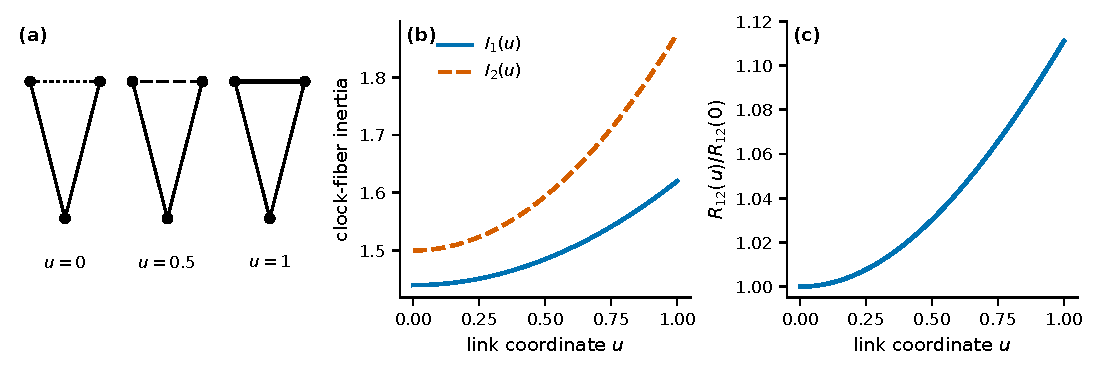
\includegraphics[width=\textwidth]{Fig1.pdf}
\caption{Connected interaction change and relative clock transport. (a) The third interaction channel is continuously activated by the nonnegative weight $u^2$ while the permanent links keep the graph connected. (b) The illustrative clock-fiber inertias change unequally. (c) The normalized relative cycle-rate ratio changes accordingly and reaches $\Xi_{+-}=1.111111$ at $u=1$.}
\label{fig:transport}
\end{figure}

Set $p_x=0$ and impose the lifted endpoint differences
\begin{equation}
\Delta z=0.5,\qquad\Delta\theta_1=0.8,\qquad\Delta\theta_2=0.55,\qquad u_-=0,\qquad u_+=1.
\end{equation}
Solving the endpoint quadratures gives
\begin{equation}
(p_z,\pi_1,\pi_2)=(1.5177135,2.2376786,1.6581369).
\end{equation}
The effective potential remains below $E_u=5$ throughout the interval, so the branch crosses from $u=0$ to $u=1$ without a turning point. The conservative orbit does not settle at $u=1$; it continues until a later turning point unless dissipation is added.

Figure~\ref{fig:transport} displays the conceptual content of the example. The closure edge is activated continuously; the two clock inertias change by unequal fractions; and the same-orbit relative cycle ratio therefore changes. The endpoint inertias are
\begin{equation}
(I_1,I_2)|_{u=0}=(1.44,1.50),\qquad (I_1,I_2)|_{u=1}=(1.62,1.875),
\end{equation}
and $\Xi_{+-}=1.111111$. These values are illustrative and are not compared with experiment.

A fixed-endpoint numerical check of the stationary-action proposition resolves the conserved charges after changing $\mu$ so that the endpoint data and winding branch remain fixed. At $\mu=0.4$, a centered finite difference with step $10^{-4}$ gives
\begin{equation}
\frac1{S_0}\left.\frac{\partial S_{\rm on}}{\partial\mu}\right|_{\rm finite\ difference}=0.35388517,
\end{equation}
while direct evaluation of the sensitivity integral gives
\begin{equation}
\frac1{S_0}\left.\frac{\partial S_{\rm on}}{\partial\mu}\right|_{\rm sensitivity\ integral}=0.35388518.
\end{equation}
The agreement verifies the envelope-theorem calculation on this regular branch; it is not evidence for a physical value of $\mu$.

\section{Interpretation, limitations, and correspondence}

\subsection{What the finite model establishes}

Within its stated domain, the model establishes four points. First, open and closed interaction organizations can be represented in one connected constrained phase space, eliminating the need for an arbitrary identification between separately calibrated theories. Second, uninterrupted transport of two specified compact clocks produces a conditional complete observable and the relative endpoint observable in Theorem~\ref{thm:transport}, with an exact no-effect condition and explicit preparation dependence. Third, persistent organization and particle non-co-motion can occupy distinct metric blocks and remain operationally distinguishable. Fourth, the stationary Jacobi action is branchwise nondecreasing in the positive co-motion-loading coefficient.

The exact Noether transport law is
\begin{equation}
\frac{\dd}{\dd\lambda}[I_i(u)\omega_i]=0,\qquad\omega_i=\frac{\dot\theta_i}{N},
\end{equation}
or equivalently
\begin{equation}
\dd\omega_i+\omega_i\dd\ln I_i=0
\end{equation}
along the orbit. This is clock-specific weighted Noether transport. It is not a new connection with nonzero curvature and does not by itself imply a universal weighted-conservation law.

\subsection{Universal fractional response and operational invisibility}
\label{sec:universal}

The universal-response surface is conceptually important because it marks the limit of what a local two-clock comparison can reveal. If every clock has
\begin{equation}
I_i(u)=I_{i0}F(u),
\end{equation}
then
\begin{equation}
R_{12\mid u}(u_*)=\frac{\pi_1I_{20}}{\pi_2I_{10}},\qquad \Xi_{+-}=1
\end{equation}
for every pair of clocks and every pair of organization surfaces on the regular branch. Each individual rate changes under uninterrupted charge transport, $\omega_i\propto F^{-1}$, but every relative clock ratio is unchanged. A purely universal multiplicative clock response is therefore operationally invisible to co-located two-clock comparisons within the closed system.

This cancellation is not evidence that $F$ is meaningless in every enlarged theory. It states the additional structure required to give it empirical content. A universal factor could become observable only through a comparison that is not transformed in the same way: for example, transport between spatially separated regions, coupling to an independently specified geometric interval or propagation sector, boundary data, or a non-clock observable with a different response. None of that additional structure is present in the finite model. Consequently, the model does not license interpreting $F(u)$ by itself as an observable scalar ``rate of time.''

Three response classes should therefore be kept distinct:
\begin{enumerate}[leftmargin=2em]
\item \emph{Universal fractional response:} $I_i=I_{i0}F$, for which all local two-clock transport signals cancel.
\item \emph{Common factor with representation weights:} $I_i=I_{i0}\Pi(u)^{w_i}$, for which
\begin{equation}
\ln\Xi_{+-}=(w_2-w_1)\Delta\ln\Pi.
\end{equation}
Only differences of weights are observable in relative clock transport.
\item \emph{Clock-specific response:} independent positive $I_i(u)$, for which the general criterion in Theorem~\ref{thm:transport} applies without a single common factor.
\end{enumerate}
The linear ansatz used here admits the common-factor form only approximately at weak coupling. A microscopic theory would have to determine whether the universal surface is an attractor, a symmetry-protected relation, or a tuning. This conclusion also constrains any continuum ``progression'' proposal: universal local rescaling alone cannot be detected by comparing two clocks that share it identically.

\subsection{What remains model dependent}

The scalar $C(u)$ is prescribed rather than microscopically derived. The phase-only reduction assumes heavy radial modes. The link coordinate and graph weights may ultimately reduce to ordinary collective coordinates and kinetic matrices of a more fundamental matter model. Unequal clock responses are parameters, not predictions for atomic, optical, nuclear, or mechanical clocks. A microscopic completion could reveal that the finite construction is a conventional entrainment or variable-inertia system expressed relationally. That outcome would preserve the consistency and observability result while removing any claim to a new fundamental mechanism.

Regularity also remains branch dependent. The model requires positive metric coefficients, $E_u>V_{\rm eff}$, and nonzero conjugate charge for whichever variable is used as a clock. Turning points terminate $u$ as a monotonic label; $p_z=0$ removes the shape clock; and compact phases cease to be global labels after one cycle unless periodic-clock data are supplied.

\subsection{Requirements for a spacetime extension}

A continuum extension would face substantially stronger requirements than the finite first-class check. It would need quasi-local interaction variables and cluster decomposition; local constraints with a hypersurface-deformation structure or an empirically equivalent alternative \cite{HKT,Bojowald}; a covariant continuum replacement of the graph form whose null directions represent common transport without a preferred frame; a stable common causal cone; and one action from which active sourcing, passive response, inertia, and clock behavior all follow. A finite Noether charge is not a local current density, stress-energy tensor, or gravitational source.

The next discriminating calculation is therefore microscopic rather than gravitational phenomenology. The prescribed closure link should be replaced by a dynamical interaction channel with reciprocal forces and radial clock modes. The effective $I_i(u)$ and active-link kinetic form should then be derived, the full coupled stability matrix tested, and the universal-response surface examined as either an attractor or a tuning.

\section{Conclusion}

A comparison between separately calibrated interaction sectors cannot by itself establish an intrinsic clock effect. Each sector may admit its own coordinate normalization, and the result depends on how endpoint canonical data are identified. The present construction answers the calibration question by placing both organizations, the particle relations, and two operationally specified compact clocks in one connected reparameterization-invariant system. The same clocks are transported without intervention, and their relative rate at selected organization surfaces is represented by a branch-local complete observable.

The novelty is not the familiar identity $I\dot\theta=\mathrm{const}$. It is the theorem that, after fixing clock identity and unit-cycle normalization, transporting the same conserved canonical data, conditioning on relational organization surfaces, and stating the preparation protocol, the cross-organization double ratio survives as a gauge-invariant observable. For arbitrary positive inertias it is nontrivial exactly when the two fibers undergo unequal fractional changes. Proposition~\ref{prop:nonremove} further shows that a nonconstant fiber circumference cannot be eliminated by a degree-one clock-preserving diffeomorphism; a covering map or a change of cycle normalization defines a different clock construction.

The comparison is not preparation independent. Uninterrupted Noether-charge transport, rate resetting, and equal-energy preparation define different physical experiments. Nor does the model make a universal factor locally visible: if all clock fibers share the same fractional response, every two-clock double ratio cancels. Such a factor could acquire operational meaning only through additional spatial, geometric, propagation, boundary, or non-clock structure not supplied here.

Persistent organization changes the clock-fiber inertias, while departure from particle co-motion enters through a positive active-link graph form. Increasing the coefficient of that form cannot decrease the stationary Jacobi action on a fixed regular branch, with equality precisely for particle co-motion modulo translation. The result is restricted but definite: interaction-dependent clock geometry and particle-co-motion loading can be represented as distinct, calculable deformations of one finite relational Jacobi system without hiding the comparison in a cross-sector calibration convention. No universal clock response, local spacetime dynamics, or gravity has been derived. Whether the structures survive microscopic derivation and continuum constraint closure remains open.

\begin{appendices}
\setcounter{figure}{1}% Continue main-text figure numbering in the appendices.
\renewcommand{\thefigure}{\arabic{figure}}
\setcounter{equation}{0}
\makeatletter
\@addtoreset{equation}{section}
\makeatother
\renewcommand{\theequation}{\thesection\arabic{equation}}
\section{Phase reduction and equations of motion}

For $\psi_i=r_i\e^{\mathrm i\theta_i}$,
\begin{equation}
\dd\psi_i^*\dd\psi_i=(\dd r_i)^2+r_i^2(\dd\theta_i)^2.
\end{equation}
The metric coefficient in the effective phase-clock ansatz reduces to $I_i(u)$ when the steep radial potential constrains $r_i$ near $r_{i0}$. Corrections are controlled by the ratio of the organization-change scale to the radial mass. The reduced einbein equations are
\begin{align}
\dot x&=N\frac{p_x}{A_x},&\dot p_x&=0,&
\dot z&=N\frac{p_z}{A_z(u)},&\dot p_z&=0,\\
\dot u&=N\frac{p_u}{K},&\dot p_u&=-N\frac{\dd V_{\rm eff}}{\dd u},&
\dot\theta_i&=N\frac{\pi_i}{I_i(u)},&\dot\pi_i&=0.
\end{align}
Combining the $u$ equation with the constraint yields the orbit quadratures.

\section{Diagonalization and curvature}

In the $(\rho,\xi)$ basis, the reduced active-link matrix is
\begin{equation}
M(u)=\frac12
\begin{pmatrix}
5+u^2 & \sqrt3(1-u^2)\\
\sqrt3(1-u^2) & 3(1+u^2)
\end{pmatrix}.
\end{equation}
Its $u$-independent orthonormal eigenvectors are the combinations defining $(x,z)$, with eigenvalues $3$ and $1+2u^2$. Hence
\begin{equation}
\det[m\mathbf1+\mu M(u)]=(m+3\mu)[m+\mu(1+2u^2)]>0.
\end{equation}
For a two-dimensional metric $\dd s^2=K\dd u^2+A(u)\dd z^2$, set $r=\sqrt K u$ and $f(r)=\sqrt{A(u(r))}$. The Gaussian curvature is $-f''/f$, yielding the curvature quoted in the text.

\section{Numerical boundary-value construction}

Using $u$ as the monotonic path parameter, collect the cyclic charges as
\begin{equation}
c=(p_z,\pi_1,\pi_2),\qquad A(u)=(A_z,I_1,I_2).
\end{equation}
Define
\begin{equation}
q_c(u)=\sum_{a=1}^3\frac{c_a^2}{2[E-V(u)]A_a(u)}.
\end{equation}
The stationary endpoint derivatives are
\begin{equation}
\frac{\dd Q_a}{\dd u}=\frac{c_a}{A_a(u)}\sqrt{\frac{K}{2[E-V(u)][1-q_c(u)]}},\qquad (Q_1,Q_2,Q_3)=(z,\theta_1,\theta_2).
\end{equation}
The charges in the numerical example solve the three endpoint equations
\begin{equation}
\Delta Q_a=\int_0^1\frac{\dd Q_a}{\dd u}\dd u.
\end{equation}
The stationary abbreviated action is
\begin{equation}
\frac{S_{\rm on}}{S_0}=\int_0^1\sqrt{\frac{2K[E-V(u)]}{1-q_c(u)}}\dd u.
\end{equation}
Figure~\ref{fig:branch} shows the effective-potential margin and the monotonic link orbit used in the numerical check.

\begin{figure}[ht]
\centering
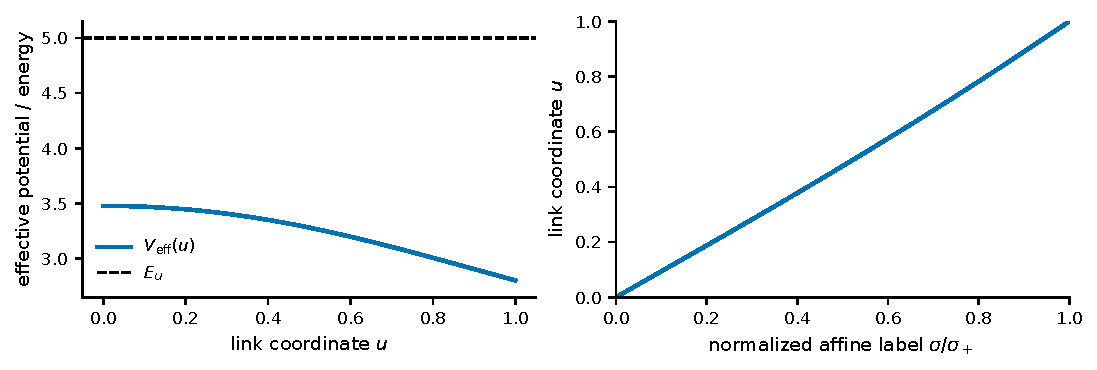
\includegraphics[width=\textwidth]{Fig2.pdf}
\caption{Representative regular branch. The effective potential stays below the available link energy, and the link coordinate is monotonic in the normalized affine label.}
\label{fig:branch}
\end{figure}

\section{Equal-energy preparation}

At fixed organization, the individual clock energy is
\begin{equation}
E_i^{\rm cl}=\frac{\pi_i^2}{2I_i}.
\end{equation}
If the individual clock energies are prepared equally in independent endpoint experiments, then $\pi_i\propto\sqrt{I_i}$ and
\begin{equation}
\frac{\omega_1}{\omega_2}\propto\sqrt{\frac{I_2}{I_1}}.
\end{equation}
The endpoint double ratio is therefore $\sqrt{\Xi_{+-}}$. If angular rates are imposed directly, the double ratio is unity. These alternatives confirm that preparation is physical input rather than gauge.

\end{appendices}

\backmatter

\section*{Supplementary information}

Online Resource 1 contains the Python source used to reproduce Figs.~\ref{fig:transport} and \ref{fig:branch}, solve the boundary-value problem for the conserved charges, calculate the endpoint transport ratio, and verify the fixed-endpoint sensitivity result.

\section*{Statements and Declarations}

\noindent\textbf{Funding.} The author received no funding for this work.

\noindent\textbf{Competing interests.} The author declares no competing financial or non-financial interests.

\noindent\textbf{Author contributions.} Scott A. Jordan conceived the model, performed the analysis and numerical calculations, and wrote the manuscript.

\noindent\textbf{Data availability.} No external datasets were used. All numerical inputs are specified in the manuscript.

\noindent\textbf{Code availability.} Source code reproducing the figures, conserved charges, endpoint transport ratio, and fixed-endpoint sensitivity check is provided as Online Resource 1.

\noindent\textbf{Use of generative AI.} During preparation of this manuscript, the author used OpenAI ChatGPT to assist with structural editing, mathematical exposition, LaTeX preparation, and figure-generation code. The author reviewed and revised all output and takes full responsibility for the content of the manuscript.

\bibliography{references}

\end{document}
